\clearpage% Flush earlier floats (otherwise order might not be correct)
\newpage


\section{Results}\label{sec:results}
This section presents a painting placement solution to the seven painting placement instances described in table~\ref{tab:instances}.

Hyperparameter values used to obtain all results in this section are in table~\ref{tab:hyperparameters-values}.
They are selected based on the hyperparameter testing from section~\ref{sec:hyper-parameters}.

The only difference is that \verb|maxNumberOfIter| is set to 500 instead of recommended range \numrange{100}{150} to possibly find better painting placement solution.
Other hyperparameters are set to their recommended values from section~\ref{sec:hyper-parameters}.
Hyperparameter \verb|populationSize| is set as the middle of the recommended range \numrange{50}{100}.
Penalization for orientation weight is removed by setting \verb|orientationWeights| to $\langle 1,1,1\rangle$.


\begin{table}[h!]
    \caption{Hyperparameter values used to obtain results}
    \label{tab:hyperparameters-values}
    \begin{threeparttable}
        \begin{tabular}{ll}
            \hline
            \textbf{Hyperparameter}                           & \textbf{Value}                                           \\ \hline
            \verb|maxNumberOfIter|                            & 500                                                      \\ \hline
            \verb|populationSize|                             & 75 times the instance size                               \\ \hline
            \verb|maximumWildCardCount|                       & 1                                                        \\ \hline
            \verb|orientationWeights|                         & $\langle 1,1,1 \rangle$                                  \\ \hline
            \verb|populationDivisionCounts|                   & remove elitism and random                                \\ \hline
            \verb|initialPopulationDivisionCounts|            & 0.7 random, 0.3 greedy                                   \\ \hline
            \verb|overlappingPenalizationConstant|            & \begin{tabular}[c]{@{}l@{}}
                                                                    two times the diagonal length\\ of the layout
            \end{tabular} \\ \hline
            \verb|outsideOfAllocatedAreaPenalizationConstant| & 0                                                        \\ \hline
        \end{tabular}
        \begin{tablenotes}
            \small
            \item Hyperparameter description is in table~\ref{tab:hyperparameters-description}.
        \end{tablenotes}
    \end{threeparttable}
\end{table}


%\afterpage{%
%    \clearpage% Flush earlier floats (otherwise order might not be correct)
%    \begin{landscape}% Landscape page
\begin{figure}[h!]
    \centering
    \subfloat[brute-force]{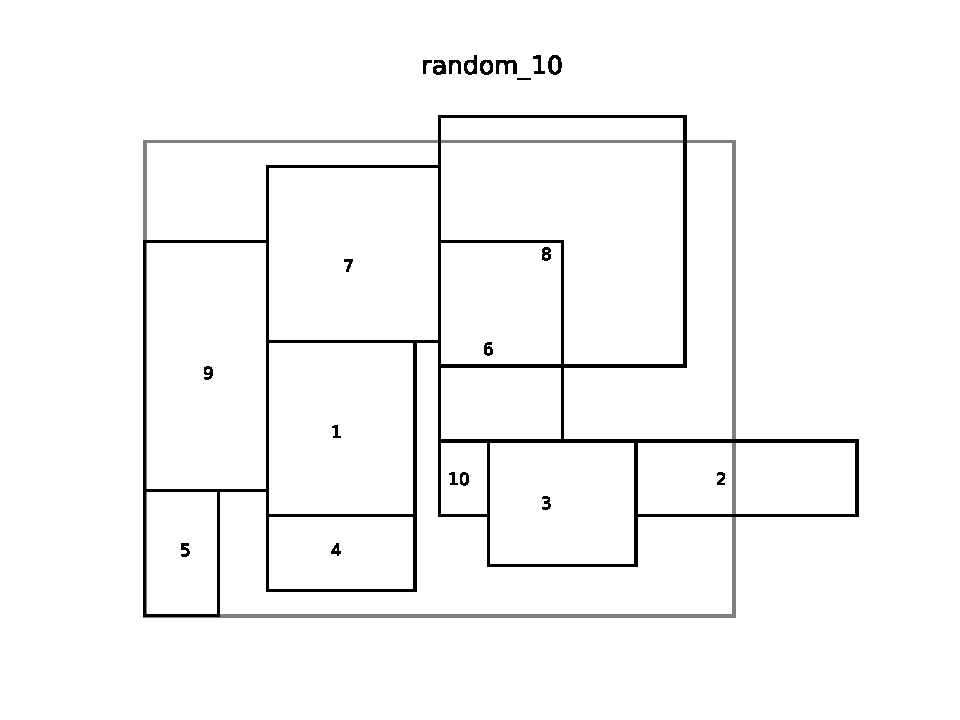
\includegraphics[width=0.9\textwidth]{visualization_random10_brute}\label{subfig:random10-brute}}

    \subfloat[proposed solution]{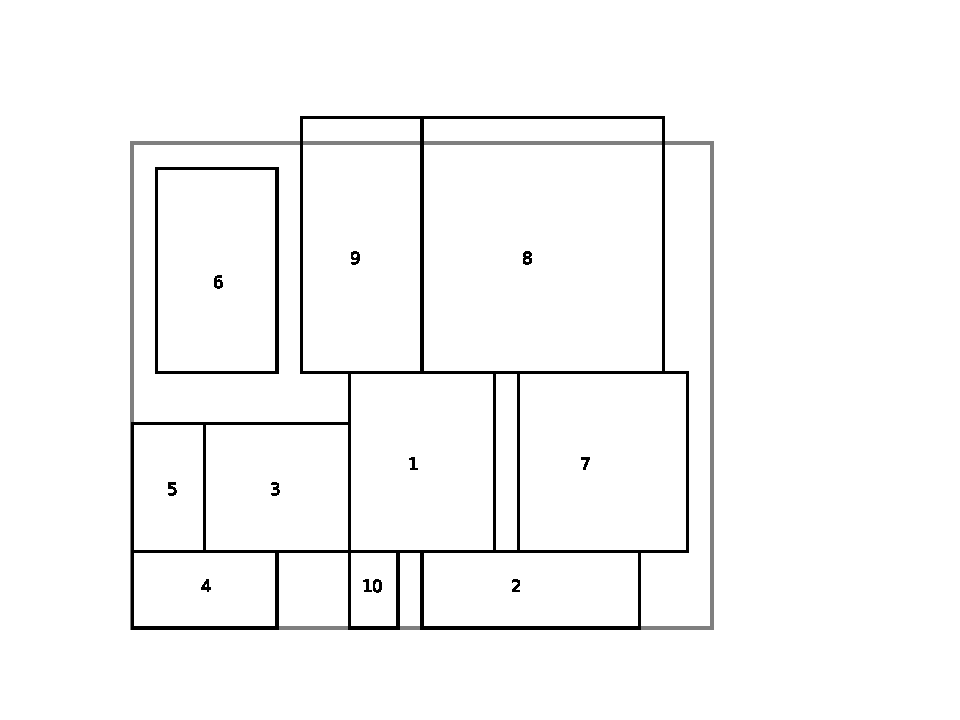
\includegraphics[width=0.9\textwidth]{visualization_random10_ga}\label{subfig:random10-ga}}
    \caption[Random\_10 instance solution visualization for brute-force]
        {Visualization of best result of proposed solution and brute-force for random\_10 instance.}
    \label{fig:visualization-random10}%
\end{figure}
%    \end{landscape}
%    \clearpage% Flush page
%}

%\afterpage{%
%    \clearpage% Flush earlier floats (otherwise order might not be correct)
%    \begin{landscape}% Landscape page
\begin{figure}[h!]
    \centering
    \subfloat[brute-force]{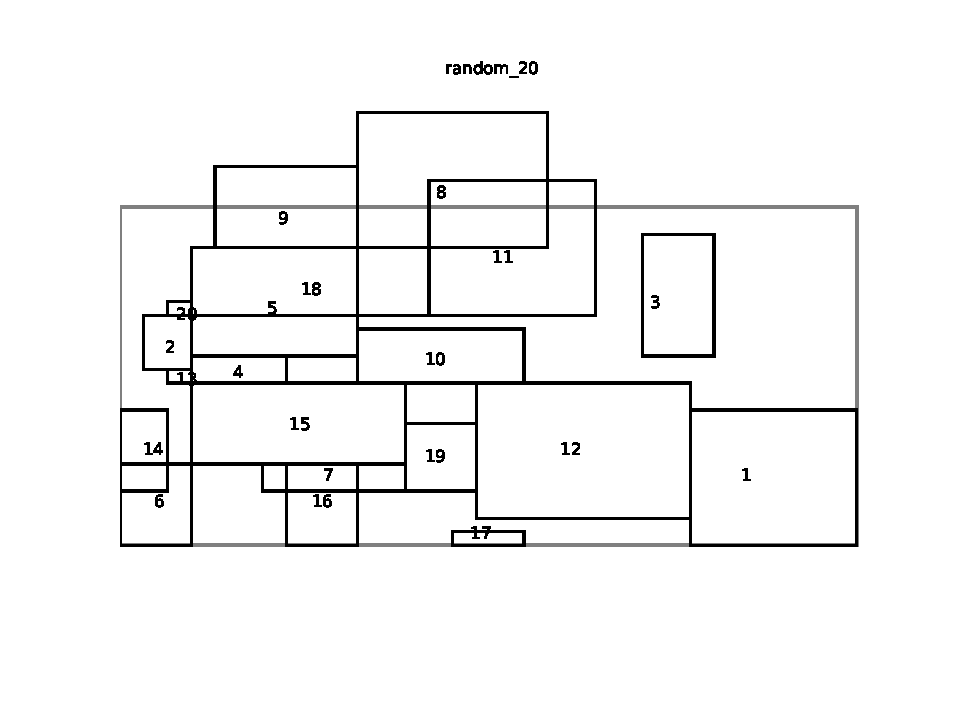
\includegraphics[width=0.8\textwidth]{visualization_random20_brute}\label{subfig:random20-brute}}

    \subfloat[proposed solution]{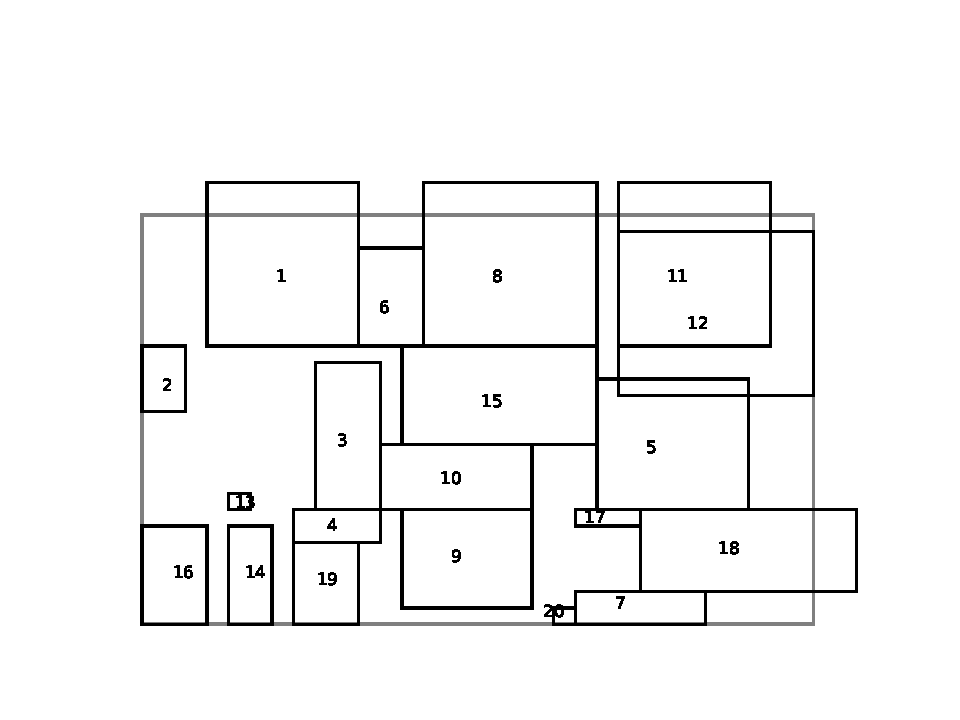
\includegraphics[width=0.8\textwidth]{visualization_random20_ga}\label{subfig:random20-ga}}
    \caption[Random\_10 instance solution visualization for proposed solution]
        {Visualization of best result of proposed solution and brute-force for random\_20 instance.}
    \label{fig:visualization-random20}%
\end{figure}
%    \end{landscape}
\clearpage% Flush page
%}

%\afterpage{%
%    \clearpage% Flush earlier floats (otherwise order might not be correct)
%    \begin{landscape}% Landscape page
\begin{figure}[h!]
    \centering
    \subfloat{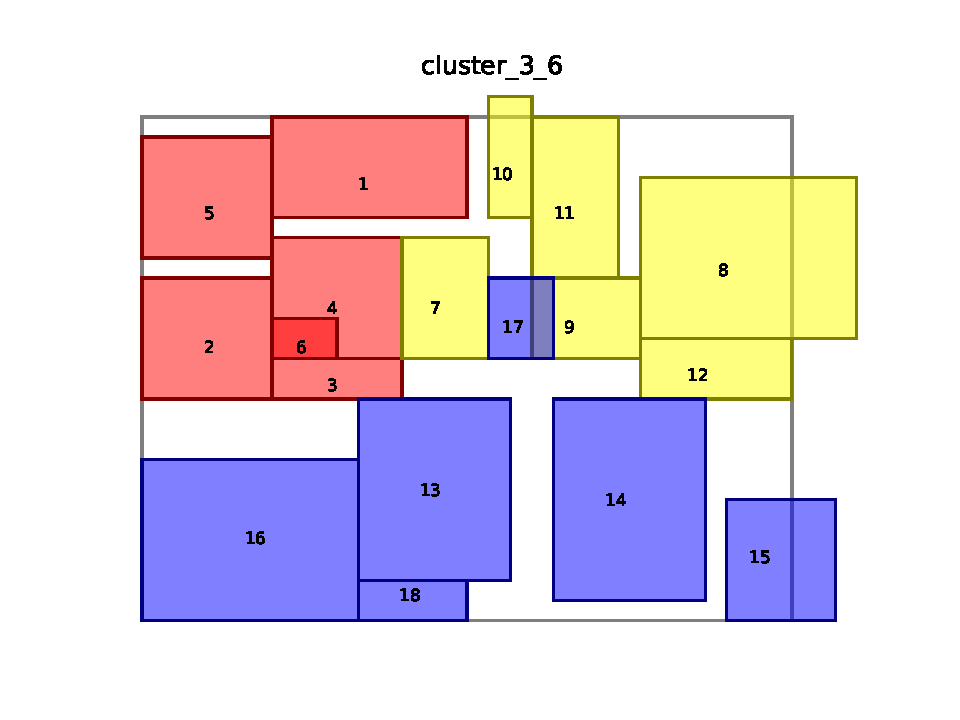
\includegraphics[width=0.8\textwidth]{visualization_cluster_3_6_ga}\label{subfig:cluster-3-6-ga}}

    \subfloat{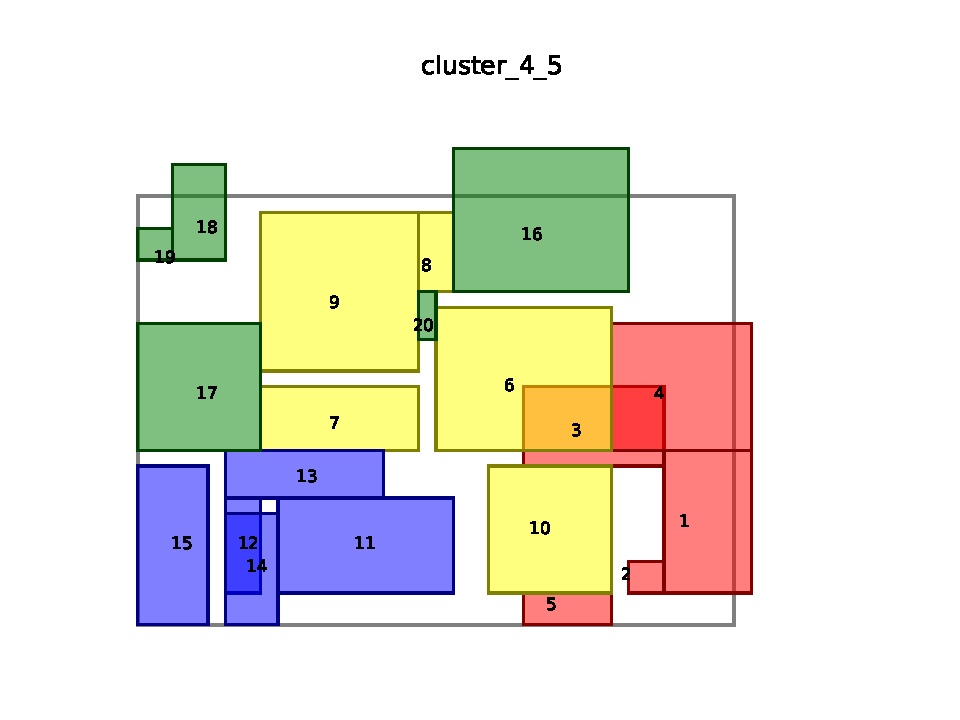
\includegraphics[width=0.8\textwidth]{visualization_cluster_4_5_ga}\label{subfig:cluster-4-5-ga}}
    \caption[Solution visualization of clustering instances for proposed solution]
    {Visualization of the best result of proposed solution for instances cluster\_3\_6 and cluster\_4\_5.}
    \label{fig:visualization-cluster}%
\end{figure}
%    \end{landscape}
%    \clearpage% Flush page
%}

%\afterpage{%
%    \clearpage% Flush earlier floats (otherwise order might not be correct)
%    \begin{landscape}% Landscape page
\begin{figure}[h!]
    \centering
    \subfloat{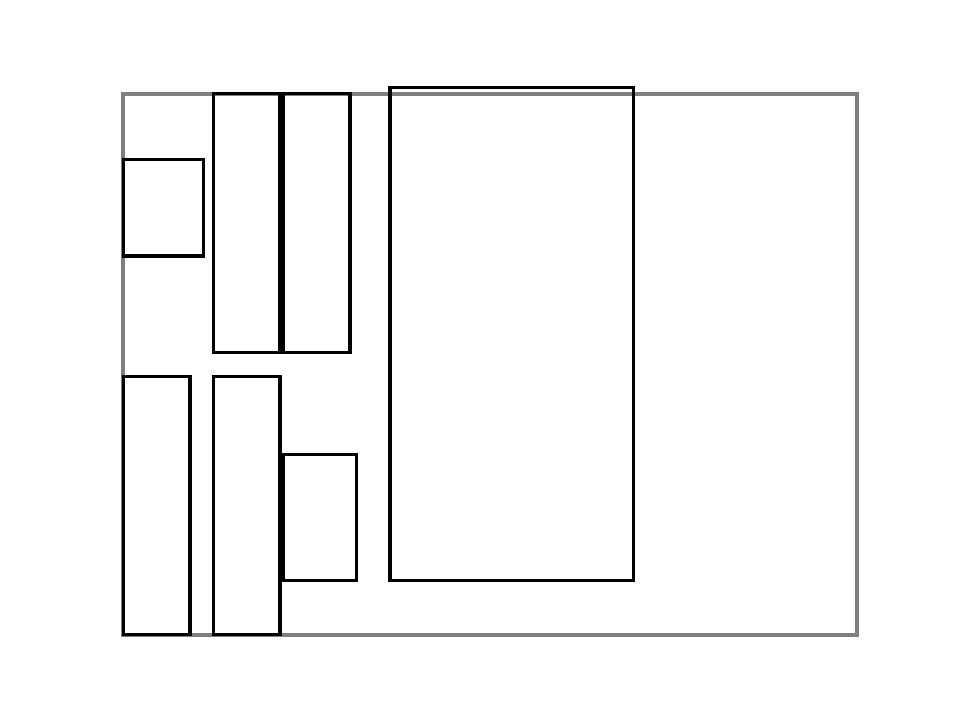
\includegraphics[width=0.8\textwidth]{visualization_london_nationa_gallery_ga}\label{subfig:london-gallery-ga}}
    \caption[London National Gallery solution visualization]
    {Visualization of the London National Gallery wall dataset.}
    \label{fig:visualization-cluster}%
\end{figure}
%    \end{landscape}
%    \clearpage% Flush page
%}
